% ----------------------------------------------------------
% DEFINITION
% ----------------------------------------------------------
\section{Definition and Mathematical Formulation}

The Forecast Readiness Score (FRS) is a composite metric designed to evaluate how
well a forecast supports operational readiness: the ability of a system to
consistently satisfy demand while avoiding economically inefficient overbuild.
FRS integrates two complementary components:

\begin{itemize}
    \item \textbf{No--Shortfall Level (NSL)}, which measures reliability, and
    \item \textbf{Cost--Weighted Service Loss (CWSL)}, which measures asymmetric
          economic cost.
\end{itemize}

By combining these perspectives—service protection and cost discipline—FRS
provides a single, interpretable measure of operational forecast quality.

\subsection{Component Definitions}

Let \(T\) denote the number of evaluation intervals. For each interval
\(t \in \{1,\dots,T\}\), let \(y_t \ge 0\) denote actual demand and
\(\hat{y}_t \ge 0\) the forecast. Let \(\cu > 0\) and \(\co > 0\) denote the
penalties for underbuild and overbuild, respectively.

\subsubsection*{(a) No--Shortfall Level (NSL)}

The No--Shortfall Level measures the fraction of intervals in which the forecast
meets or exceeds realized demand:
\[
\NSL = \frac{1}{T} \sum_{t=1}^T \indicator{\hat{y}_t \ge y_t}.
\]

By definition, \(\NSL \in [0,1]\), with higher values indicating fewer shortfall
events.

\subsubsection*{(b) Cost--Weighted Service Loss (CWSL)}

CWSL quantifies asymmetric error costs by applying different penalties to
shortfall and overbuild magnitudes. The use of asymmetric cost weighting reflects
a longstanding recognition in forecasting and decision theory that the economic
impact of overforecasting and underforecasting differs materially across
applications \citep{granger1969}.
\[
\CWSL = 
\frac{
\sum_{t=1}^T 
\left( 
    \cu \, \pospart{y_t - \hat{y}_t}
    +
    \co \, \pospart{\hat{y}_t - y_t}
\right)
}{
\sum_{t=1}^T y_t
}.
\]

CWSL is nonnegative, equals zero only for perfect forecasts, and increases with
economically meaningful deviations.

\subsection{Need for Normalization}

Because \NSL{} lies in \([0,1]\) but \CWSL{} may exceed 1, the cost term is scaled
to the unit interval to ensure comparability:
\[
\CWSLscaled 
    = \min\!\left( 1, \frac{\CWSL}{\CWSLmax} \right),
\]
where \(\CWSLmax > 0\) is a user–selected upper bound representing the largest
economically meaningful service loss for the application.

Both \NSL{} and \CWSLscaled{} now lie in \([0,1]\), enabling a bounded and
interpretable composite score.

% ----------------------------------------------------------
% FIGURE: FRS GEOMETRY (Modular)
% ----------------------------------------------------------
\begin{figure}[h!]
\centering
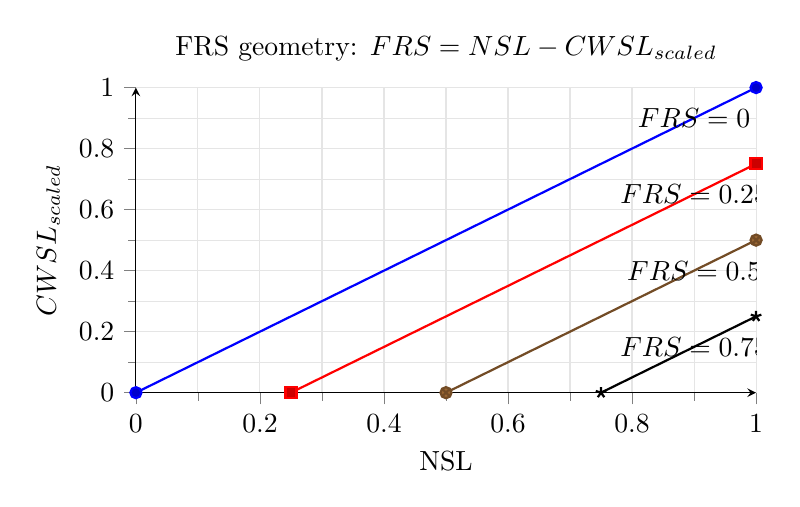
\begin{tikzpicture}

\begin{axis}[
    width=0.78\linewidth,
    height=0.45\linewidth,
    xmin=0, xmax=1,
    ymin=0, ymax=1,
    xlabel={NSL},
    ylabel={$CWSL_{\text{scaled}}$},
    axis lines=left,
    tick align=outside,
    grid=both,
    minor tick num=1,
    title={FRS geometry: $FRS = NSL - CWSL_{\text{scaled}}$},
    grid style={gray!20},
]

% Iso-FRS lines: CWSL_scaled = NSL - constant
\addplot+[domain=0:1, samples=2, thick] ({x},{x});
\addplot+[domain=0.25:1, samples=2, thick] ({x},{x - 0.25});
\addplot+[domain=0.5:1, samples=2, thick] ({x},{x - 0.5});
\addplot+[domain=0.75:1, samples=2, thick] ({x},{x - 0.75});

\node at (axis cs:0.9,0.9) {$FRS=0$};
\node at (axis cs:0.9,0.65) {$FRS=0.25$};
\node at (axis cs:0.9,0.4) {$FRS=0.5$};
\node at (axis cs:0.9,0.15) {$FRS=0.75$};

\end{axis}

\end{tikzpicture}

\caption{
FRS geometry as a function of NSL and $CWSL_{\text{scaled}}$. Diagonal level sets
represent constant values of $FRS = NSL - CWSL_{\text{scaled}}$, illustrating the
tradeoff between reliability and normalized cost.
}
\label{fig:frs_geometry}
\end{figure}

\subsection{Final Definition of the Forecast Readiness Score}

The Forecast Readiness Score is defined as:
\[
\FRS = \NSL - \CWSLscaled.
\]

Because each component lies within the unit interval, the resulting composite
satisfies:
\[
\FRS \in [-1, 1].
\]

High values of \FRS{} indicate forecasts that avoid shortfalls and exhibit low
normalized cost exposure; low or negative values indicate readiness deficits,
typically arising from shortfalls or large asymmetric errors.

\subsection{Interpretation}

\[
\begin{aligned}
\FRS \approx 1   &:& \text{excellent readiness; highly reliable and cost-efficient}, \\
\FRS \approx 0.5 &:& \text{mixed performance; moderate reliability or cost inefficiency}, \\
\FRS \approx 0   &:& \text{weak readiness; meaningful shortfall or cost exposure}, \\
\FRS < 0         &:& \text{cost-dominated regime; severe readiness deficiency}.
\end{aligned}
\]